\documentclass[12pt,letterpaper]{article}

%\usepackage{fixltx2e}
\usepackage{textcomp}
\usepackage{fullpage}
\usepackage{amsfonts}
\usepackage{verbatim}
\usepackage[english]{babel}
\usepackage{pifont}
\usepackage{color}
\usepackage{setspace}
\usepackage{lscape}
\usepackage{indentfirst}
\usepackage[normalem]{ulem}
\usepackage{booktabs}
%\usepackage{nag}
%\usepackage{natbib}
%\usepackage{bibtex}
\usepackage{float}
\usepackage{latexsym}
%\usepackage{hyperref} 
\usepackage{url}
%\usepackage{html}
\usepackage{hyperref}
\usepackage{epsfig}
\usepackage{graphicx}
\usepackage{amssymb}
\usepackage{amsmath}
\usepackage{bm}
\usepackage{array}
%\usepackage{mhchem}
\usepackage[version=4]{mhchem}
\usepackage{ifthen}
\usepackage{caption}
\usepackage{hyperref}
%\usepackage{xcolor}
\usepackage{amsthm}
\usepackage{amstext}
\usepackage{enumerate}
\usepackage{csquotes}
\usepackage{setspace}
\usepackage{longtable}
\usepackage{lscape}
\usepackage{algorithmic}

% Add and remove packages as necessary for your manuscript.
%\RequirePackage{lineno}

%\setlength{\extrarowheight}{20pt}
\linespread{1.66}
% All text should be double-spaced
% with occasional exceptions for tables. 
\raggedright
\setlength{\parindent}{0.5in}

\setcounter{secnumdepth}{0}
% Our sections are not numbered and our papers do not have
% Tables of Contents. We don't 
% present a list of figures or list of tables, either.

% Any common font is fine.
% (A common sans-serif font should be used on figures, but figures should be
% separate from the LaTeX document.)
%\pagestyle{empty}

\renewcommand{\section}[1]{%
\bigskip
\begin{center}
\begin{Large}
\normalfont\scshape #1
\medskip
\end{Large}
\end{center}}

%\renewcommand{\subsection}[1]{%
%\bigskip
%\begin{center}
%\begin{large}
%\normalfont\itshape #1
%\end{large}
%\end{center}}

%\renewcommand{\subsubsection}[1]{%
%\vspace{2ex}
%\noindent
%\textit{#1.}---}
\def\doubleq#1{``#1''}
\def\singleq#1{`#1'}

%\renewcommand{\tableofcontents}{}

%\usepackage{natbib}
%\bibpunct{(}{)}{;}{a}{}{,}  % this is a citation format command for natbib

%%% NUMBERED BIB
%\usepackage[round,numbers,sort&compress]{natbib}
%\renewcommand{\bibnumfmt}[1]{#1.}
%%% NUMBERED BIB SUPERSCRIPT
\usepackage[super,comma,sort&compress]{natbib} 
\renewcommand{\bibnumfmt}[1]{#1.}

\newcommand{\T}{{\theta}} 
\newcommand{\TP}{{\theta^{\prime}}}
\newcommand{\UB}{{\mathbf{u}}}

\newcommand{\todo}[1]{{\textcolor{red}{[#1]}}}
\newcommand{\cmt}[1]{{\textcolor{blue}{[#1]}}}
\newcommand{\ds}[1]{{\textcolor{red}{[#1]}}}
\newcommand{\rv}[1]{{\textcolor{blue}{#1}}}
\newcommand{\cdb}[1]{{\textcolor{blue}{[#1]}}}

\usepackage{lineno}

\begin{document}
\begin{flushright}
%Version dated: \today
\end{flushright}
\bigskip
\noindent 

\bigskip
\medskip
\begin{center}

\noindent{\Large \bf Age Zircon model}

\iffalse
\bigskip
\noindent {\normalsize \sc 
Daniele Silvestro$^{1,2,3,4}$,
}
\noindent {\small \it 


$^1$Department of Biology, University of Fribourg, 1700 Fribourg, Switzerland;\\
$^2$Swiss Institute of Bioinformatics, Quartier Sorge, 1015 Lausanne, Switzerland; \\
$^3$Department of Biological and Environmental Sciences, University of Gothenburg, 413 19 Gothenburg, Sweden;\\
$^4$Gothenburg Global Biodiversity Center, 413 19 Gothenburg, Sweden;\\
}
\fi
\end{center}

\vspace{1.5in}
% \clearpage
% \newpage
% \linenumbers
\subsubsection{Main model parameters}
Let us define a dataset of $N$ dated zircons from $S$ samples. We indicate with $\mathbf{z} = \{z_1, \dots, z_N\}$ the (unknown) ages of the zircons and with $\mathbf{x} = \{x_1, \dots, x_S\}$ the ages of the samples.
The samples are ordered according on their depth and we assume their age strictly follows that order such that $x_{i} > x_{i - 1}$.

The exact age of each zircon ($z_i$) is assumed to be unknown but linked to its measured age, which is expressed as a mean $\mu_i$ and a standard deviation $\sigma_i$.
The mean ages $\mu$ and a standard deviations $\sigma$ of all zircons represent the input data of the model.
Since the age of zircons can be measured based on different methods (e.g. $m \in \{1, \dots, M \}$, e.g. Zr-U-Pb, ZFT, Ar-Ar), the true age of a zircon is assumed to be further affected by the how it was measured. We compute the likelihood of the age of a zircon $i$ based on dating method $m$ as:
\begin{equation}
P(\mu_i | z_i, \sigma_i, \epsilon_m) \sim \mathcal{N}(z_i, \sigma_i + \epsilon_m)   
\end{equation}
where 
%$\eta_m \in \mathbb{R}$ is the age bias associated with the measurement method $m$ and
 $\epsilon_m \in \mathbb{R^+}$ is the bias in the estimated error of the measurement method $m$.
The parameters  $z_i, \eta_m$ and $\epsilon_m$ are considered as unknown and estimated from the data using a Bayesian algorithm.

\begin{figure}[h!]
\centering
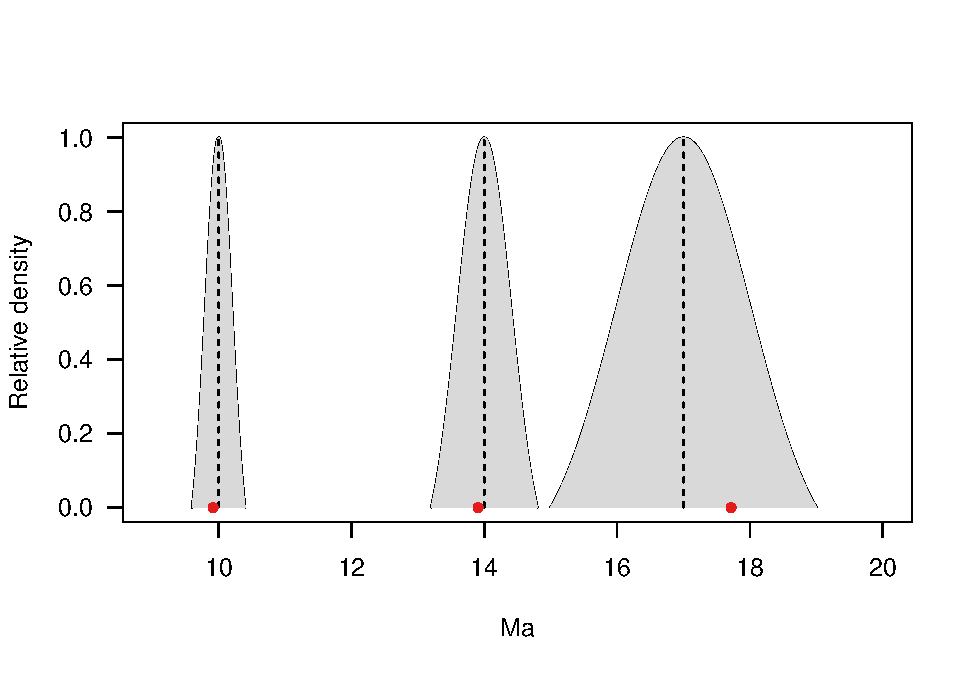
\includegraphics[width=120mm]{figs/ZirconAge.pdf}
\caption{Example of three zircons with estimated ages of 10, 14, and 17 Ma ($\mu$; indicated by the dashed vertical lines) and standard deviations ($\sigma + \epsilon$; shown by the gray shaded areas). The sampled true ages are indicated by the red circles. }
\label{f_zir_age}
\end{figure}


The prior probability of $z_{i,j}$, i.e. the $i$th zircon in sample $j$ is modeled by a half-Uniform-Cauchy distribution, which we define as
\begin{equation}
P(z_{i,j} | x_j, s_j) = \left\{
\begin{array}{@{}ll@{}}
    z_{i,j} \sim \mathcal{U}(0, 2x_j)}, & \text{if}\      z_{i,j} < x_j \\
    z_{i,j} \sim \mathcal{C}(x_j, s_j), & \text{if}\      z_{i,j} \geq x_j \\
\end{array}\right.
\end{equation}
where $x_j$ is the estimated age of the sample and $s_j$ is a sample-specific scale parameter of the Causchy distribution. 

\begin{figure}[h!]
\centering
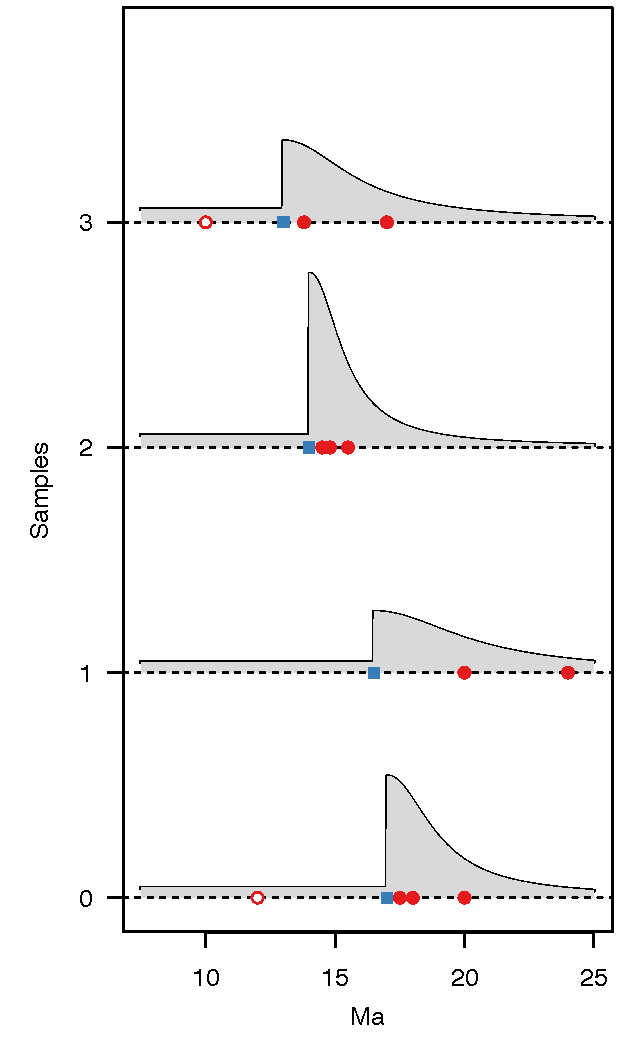
\includegraphics[width=120mm]{figs/SampleProb.pdf}
\caption{Example of three zircons with estimated ages of 10, 14, and 17 Ma ($\mu$; indicated by the dashed vertical lines) and standard deviations ($\sigma + \epsilon$; shown by the gray shaded areas). The sampled true ages are indicated by the red circles. }
\label{f_sample_prob}
\end{figure}


The value of $x_j$, the sample age, is determined by two latent variables and constrained by sampled values of $\mathbf{z}$ such that $x_{i} > x_{i - 1}$ for $i \in \{2, \dots, S\}$.
Specifically we define as 
\begin{equation}
\zeta_j = \min(z_{n}), \text{ for } n \in \{j, \dots, N\},
\end{equation}
the minimum age across all zircons included in sample $j$ and in all older samples. 
Thus, $\zeta_j$ represents the maximum boundary for the age of sample $j$.
Under this notation we define the age of a sample as: 
\begin{equation}
x_j = \left\{
\begin{array}{@{}ll@{}}
    r_j (\zeta_j), & \text{if}\ j = 1 \\
    x_{j - 1} + r_j (\zeta_j - x_{j - 1}), & \text{if}\ j > 1 \\
\end{array}\right.
\end{equation}
where $r_j \in (0, 1)$ is a sample-specific latent parameter determining how close $x_{j}$ is to its lower boundary $x_{j - 1}$ (or 0 if $j = 1$). 
%
We also account for the fact that a zircon can be younger then the sample it is assigned to, due to dating error or a later recrystallization of the zircon. 
To do that, we additionally sample a vector of identifiers $\mathbf{I} = \{I_1, \dots, I_N\}$ that define which zircons are accounted for ($I = 1$) or excluded ($I = 0$) in determining the maximum boundary for the age of sample $j$:
\begin{equation}
\zeta_j = \min(z_{n}), \text{ for } n \in \{j, \dots, N \}, \text{ if } z_j = 1.
\end{equation}

\subsubsection{Priors and hyper-priors}
We use a gamma prior for the vector of scale parameters of the Cauchy distributions $\{s_1, \dots, s_S \} \sim \Gamma(5, 5)$, a normal prior centered on 0 on the vector of bias parameters $\{\eta_1, \dots, \eta_M \} \sim \mathcal{N}(0, 5)$ and a gamma prior on the vector of parameters $\{\epsilon_1, \dots, \epsilon_M \} \sim \mathcal{N}(0, 5)$.
We use a beta distribution as prior on the vector of parameters $\{r_1 \dots, r_S\} \sim \mathcal{B}(a, b)$ and consider the shape parameters $a$ and $b$ themselves as unknown parameters and assign them gamma distributed hyper-priors, $a, b \sim \Gamma(1, 0.1)$.
Finally we use a Bernoulli distribution as prior on the indicators $\{I_1, \dots, I_N\}$ with parameter $p = 0.99$, thus assigning a 0.01 prior probability for a zircon to be younger than the sample it is assigned to. 

\subsubsection{Parameter estimation}
The model includes $2N + 2M + 2S + 2$ parameters ($z$ and $I$, $\eta$ and $\epsilon$, $s$ and $r$, $a$ and $b$, respectively). 
All parameters are estimated through Metropolis-Hastings Markov chain Monte Carlo (MCMC). We use a sliding window proposal with reflection at the boundaries for $r$, normal kernel proposals for $z$, binomial proposals for $I$ and sliding window for $\eta$. We use multiplier proposals on all other parameters since they only span the positive range. 


\end{document}
